% =====================================================================
%  c25 —— 原文印刷页 200--210（PDF 第 201--211 页）
%  含：附录 G 的 G.2（自旋与 Pin 结构的阻碍）、G.3（四维流形上的 Spin^c 结构）、
%      G.4（'t Hooft 磁通）；附录 H（联络、平行移动与和乐）之开头，至 (H.35) 止
%  编号公式：G.3--G.23（其中 (G.9) 是原稿的一条空白编号行）与 H.1--H.35，共 56 条
%  插图：Fig. 35（印刷第 207 页）、Fig. 36（印刷第 209 页）
%  全部公式均逐条对照 150 dpi 页面图像转写（文本层仅供读散文）
% =====================================================================

% 说明：本片段从 G.1 的编号列表第 4 条中间切入（G.1、G.2 在上一片段 c24 中），
%  故开头是一句残句，此处不补 \section{G} 标题。

……丛 $P$ 到 $\widetilde{G}$ 的（结构群）约化，等同于一个覆盖 $P$ 的主 $\widetilde{G}$ 丛 $\widetilde{P}$：

\begin{equation}
  \widetilde{P} \to P \to M
  \tag{G.3}
  \label{eq:G.3}
\end{equation}

使得每一点 $m\in M$ 上方的纤维「看起来像」覆盖

\begin{equation}
  1 \to K \to \widetilde{G} \to G \to 1
  \tag{G.4}
  \label{eq:G.4}
\end{equation}

\begin{enumerate}[start=5]
  \item 定向流形上\emph{自旋结构}（spin structure）的选取，是前述注记 \eqref{eq:G.2} 在
    $\phi:\mathrm{Spin}(n)\to SO(n)$ 这一情形下的特例。为了对自旋结构分类，我们先按
    $z\in H^1(\mathcal{B}_{SO}(M);\mathbb{Z}_2)$ 对 $\mathcal{B}_{SO}(M)$ 上的主 $\mathbb{Z}_2$ 丛分类。
    自旋结构就是那些限制到纤维上给出二重覆盖 $\mathrm{Spin}(n)\to SO(n)$ 的丛。二重覆盖
    $\mathrm{Spin}(n)\to SO(n)$ 对应于 $z_s\in H^1(SO(n);\mathbb{Z}_2)\cong\mathbb{Z}_2$。
    因此，自旋结构就是 $\mathcal{B}_{SO}(M)$ 的那些二重覆盖：它们限制到纤维
    $\mathcal{B}_{SO}(M)\to M$ 上给出类 $z_s$。注意两个自旋结构之差 $z_1-z_2$ 于是在纤维上是平凡的，
    从而拉回自 $H^1(M;\mathbb{Z}_2)$ 中的某个类。于是 $M$ 上的自旋结构构成
    $H^1(M;\mathbb{Z}_2)$ 的一个 torsor（主齐性空间）。

  \item 用同样的办法可以处理其它结构。对流形 $M$，基于把上述概念施用于同态
    \begin{equation}
      \phi : \mathrm{Pin}^c \to O(n)
      \tag{G.5}
      \label{eq:G.5}
    \end{equation}
    \begin{equation}
      \phi : \mathrm{Spin}^c \to O(n)
      \tag{G.6}
      \label{eq:G.6}
    \end{equation}
    \begin{equation}
      \phi : \mathrm{Pin}^{\pm} \to O(n)
      \tag{G.7}
      \label{eq:G.7}
    \end{equation}
    \begin{equation}
      \phi : \mathrm{Spin} \to O(n)
      \tag{G.8}
      \label{eq:G.8}
    \end{equation}
    \begin{equation}
      \tag{G.9}
      \label{eq:G.9}
    \end{equation}
    我们便可以谈论 $\mathrm{Pin}^c$、$\mathrm{Spin}^c$、$\mathrm{Pin}^{\pm}$、$\mathrm{Spin}$ 结构。
    注意这些同态一般既不是单射也不是满射。对于定向流形上的 BLOTZ 结构，我们把类似的同态施用于
    定向标架丛，即取值到 $SO(n)$。

    % 说明：原文 (G.9) 只有编号、没有公式体，是作者删掉一条式子后留下的空白编号行；
    %  此处照原样保留空公式，编号 G.10 及以后仍与页面图像一致。另：原文的 "BLOTZ structure"
    %  是一个未定义的占位词（字母串），疑为作者留给自己的结构名占位（按上下文应是某种
    %  twisted Pin/Spin 结构），不要擅自改写成 "Bloch"。
\end{enumerate}

\subsection{自旋与 Pin 结构的阻碍} % 原文: G.2 Obstructions To Spin And Pin Structures

把上面略嫌抽象的表述翻译成流形 $X$ 的切丛的转移函数的语言，是值得做的。设
$\{\mathcal{U}_{\alpha\beta}\}$ 是 $X$ 的坐标图册。利用度规我们可以取正交标架，若
$\dim_{\mathbb{R}}X=n$，它们有转移函数

\begin{equation}
  g_{\alpha\beta} : \mathcal{U}_{\alpha\beta} \to O(n)
  \tag{G.10}
  \label{eq:G.10}
\end{equation}

若我们能用一个上链把它们修改为

\begin{equation}
  \tilde{g}_{\alpha\beta} = h_\alpha g_{\alpha\beta} h_\beta^{-1}
  \tag{G.11}
  \label{eq:G.11}
\end{equation}

其中 $h_\alpha:\mathcal{U}_\alpha\to O(n)$，使得 $\tilde{g}_{\alpha\beta}:\mathcal{U}_{\alpha\beta}\to SO(n)$，
则流形是可定向的。可定向性的唯一阻碍由 Cech 2-上链
$\det g_{\alpha\beta}:\mathcal{U}_{\alpha\beta}\to\mathbb{Z}_2$ 提供，它定义上同调类
$w_1(X)\in H^1(X;\mathbb{Z}_2)$。注意若 $X$ 单连通，则 $H^1(X;\mathbb{Z}_2)=0$，因而它必定可定向。

% [Tutor Note: 指标个数与上链次数的错位是这一段最易读错的地方。Cech 理论中，以
%  $p+1$ 个开集为下标的族是一个 $p$-上链，所以以 $\alpha\beta$ 两个下标标注的
%  $\det g_{\alpha\beta}$ 是 1-上链、给出 $H^1$ 中的 $w_1$；而下面 (G.12) 中以
%  $\alpha\beta\gamma$ 三个下标标注的 $\xi_{\alpha\beta\gamma}$ 虽是「3-上链」（three indices），
%  它对应的却是 $H^2$ 中的 $w_2$。原文把后者称为 "Cech 3-cocycle"，指的是三个下标，
%  不是三次上同调。]

当 $X$ 可定向时，我们可以取 $g_{\alpha\beta}:\mathcal{U}_{\alpha\beta}\to SO(n)$。若选取\emph{良覆盖}
（good cover），即所有交 $\mathcal{U}_{\alpha\beta\cdots}$ 都是可缩的，则在每个重叠
$\mathcal{U}_{\alpha\beta}$ 上我们可以选取提升
$\tilde{g}_{\alpha\beta}:\mathcal{U}_{\alpha\beta}\to\mathrm{Spin}(n)$。唯一的问题是这样提升之后
上链条件可能失效。由于我们已取定提升，而覆盖 $\mathrm{Spin}(n)\to SO(n)$ 的核恰是群
$\{\pm1\}$，我们可以确知在 $\mathcal{U}_{\alpha\beta\gamma}$ 上

\begin{equation}
  \tilde{g}_{\alpha\beta}(x)\tilde{g}_{\beta\gamma}(x)\tilde{g}_{\gamma\alpha}(x)
  := \xi_{\alpha\beta\gamma}\in\{\pm1\}\subset \mathrm{Spin}(n)
  \qquad \forall x\in\mathcal{U}_{\alpha\beta\gamma}
  \tag{G.12}
  \label{eq:G.12}
\end{equation}

符号 $\xi_{\alpha\beta\gamma}$ 定义一个 Cech 3-上链，它定义 $H^2(X;\mathbb{Z}_2)$ 中的一个上同调类。
这是 $w_2$ 的一个（非常具体的）定义。注意：把提升 $g_{\alpha\beta}$ 乘上一个上链而作任意修改，
或者取不同的提升 $\tilde{g}_{\alpha\beta}$，都只把 $\{\xi_{\alpha\beta\gamma}\}$ 改变一个上边界。
几乎按定义，这就是自旋结构存在的唯一阻碍。

\begin{enumerate}
  \item 最简单的非平凡例子是圆上的自旋结构。圆是一维的，故取 $n=1$。此时 $SO(1)$ 是平凡群，
    而 $\mathrm{Spin}(1)\cong\mathbb{Z}_2$。于是圆上的自旋结构字面上就是圆的二重覆盖。这样的覆盖有两个：
    平凡的一个与非平凡的一个。在物理中它们分别称为 \emph{Neveu-Schwarz} 与 \emph{Ramond} 自旋结构。
    注意平凡的二重覆盖可以延拓为圆盘的二重覆盖，但圆的非平凡二重覆盖不能延拓到圆盘上。

    令人有些困惑的是：相对于某个自然的平凡化，Neveu-Schwarz 自旋结构中的旋量应看成圆上的
    反周期函数，而 Ramond 自旋结构中的旋量应看成周期函数。看清这一点的一个办法是直接考虑
    圆盘上的欧氏度规，取正交标架 $e_1=dr$、$e_2=rd\theta$。此时 $\omega_{12}=-d\theta$ 就是自旋联络。
    现在考虑协变旋量方程

    \begin{equation}
      D_\mu\psi = \partial_\mu\psi + \frac{1}{4}\omega_\mu^{ab}\gamma^{ab}\psi = 0
      \tag{G.13}
      \label{eq:G.13}
    \end{equation}

    而在圆盘上的自旋丛中我们可以取常旋量表示

    \begin{equation}
      \gamma^1 = i\sigma^1 \qquad \gamma^2 = i\sigma^2
      \tag{G.14}
      \label{eq:G.14}
    \end{equation}

    于是普遍的协变旋量为

    \begin{equation}
      \psi = \left( c_1 e^{-i\theta/2}\begin{pmatrix} 1 \\ 0 \end{pmatrix}
        + c_2 e^{i\theta/2}\begin{pmatrix} 0 \\ 1 \end{pmatrix} \right)
      \tag{G.15}
      \label{eq:G.15}
    \end{equation}

    % [Tutor Note: (G.13) 的因子 $1/4$ 与 $e^{\mp i\theta/2}$ 的相位要一起核对：
    %  $\gamma^{ab}=\frac12[\gamma^a,\gamma^b]$，$\omega_{12}=-d\theta$，故
    %  $\frac14\omega_\mu{}^{12}\gamma_{12}$ 中的 $\frac14$ 实际抵消了 $\gamma_{12}$ 定义里的 $\frac12$，
    %  最后给出 $\mp\frac{i}{2}\dot\theta$，积分后正是 $\mp i\theta/2$。若漏掉 $\frac12$
    %  就会得到整数相位的「旋量」，从而把 Neveu-Schwarz 与 Ramond 两种结构搞混。]

    {\small\itshape ［原文标记：这一点仍然令人困惑，因为这些波函数并不延拓到圆盘上；上面的旋量函数是相对于
    $K^{1/2}$ 的一个不延拓到圆盘上的平凡化而言的。仍需更完整地解释。Witten 关于超弦微扰论的工作中
    也许有些好的评论。］}

    % [原文待办标记，原文 p.201--p.202：作者用一行星号围出的大段自注，跨页收尾；
    %  星号内文字保留原意译出。]

    {\small\itshape ［原文标记：下面两个例子都假定 $X$ 是四维的］}

    % [原文待办标记，原文 p.202 右侧页边 \ensuremath{\clubsuit}…\ensuremath{\clubsuit} 注]

  \item 一个例子：$\mathcal{B}SO(2)=\mathcal{B}U(1)=\mathbb{C}P^\infty$。$w_2$ 是 $c_1$ 的模二约化，
    而 $c_1$ 是与 2-胞腔对偶的上链。所以请解释为什么 $c_1\bmod 2$ 是自旋结构的阻碍。在
    $\mathbb{C}P^2$ 上 $c_1=3x$。复化切丛允许把
    $SO(4)=SU(2)\times SU(2)/\mathbb{Z}_2$ 的结构群约化到
    $U(2)=SU(2)\times U(1)/\mathbb{Z}_2$。限制到 $\mathbb{C}P^1\subset\mathbb{C}P^2$ 上，切丛分裂为
    $\mathcal{O}(2)\oplus\mathcal{O}(1)$，其中 $\mathcal{O}(2)$ 是 $\mathbb{C}P^1$ 的切丛，
    而 $\mathcal{O}(1)$ 是法丛。结构群进一步约化到 $U(1)\times U(1)$。显然，与法丛
    $\mathcal{O}(1)$ 相伴的主 $U(1)$ 丛不容许一个二重覆盖，使其在 $U(1)$ 上限制为 $U(1)$ 的二重覆盖。

  \item 对 $\mathrm{Spin}^c$ 结构的阻碍是 $W_3$，即 $w_2$ 在 Bockstein 映射下的像。因此当
    $w_2(X)\in H^2(X;\mathbb{Z}_2)$ 具有整提升时它为零。利用对一切 $\sigma\in H_2(X;\mathbb{Z})$ 有

    \begin{equation}
      \int_\sigma w_2(X) = \sigma\cdot\sigma \ \ \mathrm{mod}\ 2
      \tag{G.16}
      \label{eq:G.16}
    \end{equation}

    其中 $\sigma\cdot\sigma$ 是定向整相交数，便可以证明这样的整提升确实存在。细节见 [?]。
    在不可定向的情形下类似的命题不成立：$\mathbb{R}P^2\times\mathbb{R}P^2$ 不容许
    $\mathrm{Pin}^c$ 结构。此外，还存在非 $\mathrm{Spin}^c$ 的定向五维流形。一个简单的例子是
    对称 $SU(3)$ 矩阵构成的空间，它微分同胚于 $SU(3)/SO(3)$。解释见 [?]。

    % [Tutor Note: (G.16) 左边是对 2-维闭链 $\sigma\in H_2(X;\mathbb{Z})$ 积分，右边是相交数，
    %  两者都是整（或模 2）量，但只有在 $X$ 定向且四维时 $\sigma\cdot\sigma$ 才有定义——
    %  这正是作者在旁边标注「下面两个例子假定 $X$ 四维」的原因。$W_3=\beta(w_2)$（Bockstein），
    %  不是另一个 Stiefel-Whitney 类，别把 $W_3$ 与 $w_3$ 混淆：$w_3$ 属于 $H^3$，而
    %  $W_3\in H^3(X;\mathbb{Z})$ 是 $w_2$ 的整 Bockstein 提升，其消失才是 $\mathrm{Spin}^c$ 存在的判据。]

    {\small\itshape ［原文标记：另见 Gompf、Stipsicz《4-Manifolds and Kirby Calculus》中的证明］}

    % [原文待办标记，原文 p.202 右侧页边 \ensuremath{\clubsuit}Also look up proof in Gompf, Stipszic … \ensuremath{\clubsuit}]

    {\small\itshape ［原文标记：给出证明。］}

    % [原文待办标记，原文 p.202 右侧页边 \ensuremath{\clubsuit}Give proof. \ensuremath{\clubsuit}，紧接在「五维流形」一句旁]
\end{enumerate}

\subsection{四维流形上的 $\mathrm{Spin}^c$ 结构} % 原文: G.3 Spin^c Structures On Four-Manifolds

群 $\mathrm{Spin}^c(4)$ 定义为

\begin{equation}
  \mathrm{Spin}^c(4) := \left(\mathrm{Spin}(4)\times U(1)\right)/\mathbb{Z}_2
  = \left(SU(2)\times SU(2)\times U(1)\right)/\mathbb{Z}_2
  \tag{G.17}
  \label{eq:G.17}
\end{equation}

其中我们除以按 $(-1,-1,-1)$ 嵌入的群 $\mathbb{Z}_2$。$X$ 的定向正交标架丛 $OrFr(X)$ 是主 $SO(4)$ 丛，
而自旋 $c$ 结构——按定义——是结构群到由显然同态 $\mathrm{Spin}^c(4)\to SO(4)$ 所定义的主
$\mathrm{Spin}^c(4)$ 丛的约化。把定义写开就意味着：自旋 $c$ 结构由一个主 $\mathrm{Spin}^c(4)$ 丛
$\mathfrak{P}$ 连同投影 $\mathfrak{P}\to OrFr(X)$ 给出，该投影沿着纤维看起来像正合列

\begin{equation}
  1 \to U(1) \to \mathrm{Spin}^c(4) \to SO(4) \to 1
  \tag{G.18}
  \label{eq:G.18}
\end{equation}

当 $w_2(X)$ 具有整提升时，自旋 $c$ 结构存在。如上所述，对每个紧定向四维流形这确实成立。

由 $[(v_L,v_R,\zeta)]\mapsto(\zeta v_L,\zeta v_R)$ 给出的群同态
$\mathrm{Spin}^c(4)\to U(2)\times U(2)$ 定义一个同构

\begin{equation}
  \mathrm{Spin}^c(4) \cong \left\{ (u_L,u_R)\mid \det u_L = \det u_R \right\}
  \subset U(2)\times U(2)
  \tag{G.19}
  \label{eq:G.19}
\end{equation}

后一表述使下面这件事变得显然：$\mathrm{Spin}^c(4)$ 有两个不等价的秩 2 表示 $W^{\pm}$，
它们就由两个 $U(2)$ 因子的基本表示定义。给定一个自旋 $c$ 结构，于是有两个相伴的复秩二丛
$W^{\pm}\to X$，并且在上面{\small\itshape ［原文标记：section ??（章节交叉引用待补，原稿占位符）］}
的讨论中我们可以认定

% [原文标记：原文此处写 "in the discussion of section ?? above"，章节号是作者留的占位符，
%  至今未填；对照 p.203 的上下文应是指前面讨论 Dirac 旋量丛 $S^\pm$ 与线丛 $L$ 的那一节。]

\begin{equation}
  W^{\pm} = S^{\pm}\otimes L
  \tag{G.20}
  \label{eq:G.20}
\end{equation}

反之，这样一对丛 $W^{\pm}$ 定义一个自旋 $c$ 结构。因此自旋 $c$ 结构的空间是线丛群的一个 torsor：
因为给定线丛 $\mathcal{L}$，我们总可以取

\begin{equation}
  W^{\pm} \to W^{\pm}\otimes\mathcal{L}
  \tag{G.21}
  \label{eq:G.21}
\end{equation}

使得

\begin{equation}
  c_1(\det W^{\pm}) \to c_1(\det W^{\pm}) + 2c_1(\mathcal{L})
  \tag{G.22}
  \label{eq:G.22}
\end{equation}

注意：给定 $X$ 上的近复结构，就有一个典范的自旋 $c$ 结构

\begin{equation}
  W^{+} = \Omega^{0,0}(X)\oplus\Omega^{0,2}(X)
  \qquad\qquad
  W^{-} = \Omega^{0,1}(X)
  \tag{G.23}
  \label{eq:G.23}
\end{equation}

% [Tutor Note: (G.22) 中的因子 2 不能漏。(G.20) 说 $W^{\pm}=S^{\pm}\otimes L$ 且
%  $\det S^{\pm}=1$（$S^{\pm}$ 是 $SU(2)$ 的秩 2 丛），故 $\det W^{\pm}=L^{2}$，于是
%  $\det W^{\pm}$ 的行列式线丛在 $L\to L\otimes\mathcal{L}$ 下按 $L^2\to L^2\otimes\mathcal{L}^2$
%  变换，正是 (G.22)。这也解释了自旋 $c$ 结构的 torsor 结构为何是「线丛群」而不是
%  「$H^2$ 的元素」：$L$ 与 $L\otimes\mathcal{L}$ 给出不同但同伦等价的 $W^{\pm}$。]

\subsection{'t Hooft 磁通} % 原文: G.4 ’t Hooft Flux

在讲义的好几处，我们用到主 $SO(3)$ 丛 $P$ 的第二 Stiefel-Whitney 类 $w_2(P)$。一般地，
流形 $M$ 上的 $SO(n)$ 丛 $P$ 有一个特征类 $w_2(P)\in H^2(M;\mathbb{Z}_2)$。定义它的一种办法
沿用上面关于自旋结构的讨论：选取 $M$ 的良覆盖 $\{\mathcal{U}_\alpha\}$ 以及 $P$ 在该覆盖上的平凡化。
在重叠 $\mathcal{U}_{\alpha\beta}$ 上选取提升
$\tilde{g}_{\alpha\beta}:\mathcal{U}_{\alpha\beta}\to\mathrm{Spin}(n)$，并度量上链条件在
$\mathcal{U}_{\alpha\beta\gamma}$ 上失效的程度，从而定义 $H^2(M;\mathbb{Z}_2)$ 中的一个类。
若 $w_2(P)$ 非零，则 $P$ 的结构群不能从 $SO(n)$ 约化到 $\mathrm{Spin}(n)$。

不能提升为 $\mathrm{Spin}(n)$ 丛的 $SO(n)$ 丛的一个简单例子如下：取 $M$ 为二维紧曲面。
选一点 $p\in M$ 以及 $p$ 周围的小圆盘。用绕圆盘边界的转移函数在 $SO(n)$ 中定义一条非平凡闭路，
以此定义一个 $SO(n)$ 丛。

\section{联络、平行移动与和乐} % 原文: H. Connections, Parallel Transport, And Holonomy

\begin{keytakeaways}
  \item 联络的路径提升定义：沿路径 $x(t)$ 解一阶线性 ODE
    $\frac{d}{dt}\vec{v}=A(x(t))\dot{x}\vec{v}$，其解算子就是路径排序指数
    $\mathbb{U}(\wp_t)=\mathrm{Pexp}\int_0^t A(x(t_1))\dot{x}_1dt_1$，它只依赖 $A$ 沿该路径的取值
    （而与重参数化 $t\to f(t)$、$f'>0$ 无关）。
  \item 乘法律的方向：路径提升 $\mathbb{P}$ 对复合协变，$\mathbb{P}(\wp_1\star\wp_2)=\mathbb{P}(\wp_1)\star\mathbb{P}(\wp_2)$；
    而矩阵解 $\mathbb{U}$ 对复合\emph{反变}，$\mathbb{U}(\wp_1\star\wp_2)=\mathbb{U}(\wp_2)\mathbb{U}(\wp_1)$。
    这是路径排序指数最常被记反的约定。
  \item 单值性即曲率：小环路 $\mathbb{U}(\wp)=1+\alpha F_{z\bar z}(z_0,\bar z_0)+O(\epsilon^3)$，
    其中 $\alpha$ 是环路所围面积的两倍，一般的实坐标版本是
    $\mathbb{U}(\wp)=1-\epsilon_1\epsilon_2F_{\mu\nu}(\vec{x}_0)+\cdots$。
  \item 平坦联络（$F=0$）的单值性只依赖路径的同伦类：把同伦映射的 $I^2$ 剖分成足够小的方块，
    每块的环路单值性平凡，故整体平凡。
  \item 联络是 1-形式：换坐标时必须用 $\tilde{A}(z)dz=A(x)dx$ 而非 $\tilde{A}(z)=A(x)$ 来定义，
    即 $\tilde{A}(z)=\frac{1}{2\pi i}e^{-2\pi ix}A(x)$；规范变换律为
    $A=g^{-1}\widetilde{A}g+g^{-1}dg$。
\end{keytakeaways}

{\small\itshape ［原文标记：用路径提升性质给出联络的定义］}

% [原文待办标记，原文 p.203：作者以待办口吻写的缺节提示，用星号行围出，星号行跨页至
%  p.204 顶部才收尾；星号行内的 "Our convention for concatenating curves" 与 (H.1)
%  是正文内容，故按普通正文排出。]

我们拼接曲线的约定是：

\begin{equation}
  f_1 \star f_2(t) :=
  \begin{cases}
    f_1(2t) & 0\le t\le \tfrac12 \\[2pt]
    f_2(2t-1) & \tfrac12\le t\le 1
  \end{cases}
  \tag{H.1}
  \label{eq:H.1}
\end{equation}

% [原文标记：星号行在同一待办块内跨页，p.204 顶部以一行星号收尾；此后正文接续。]

对于主丛与向量丛，我们可以把该性质用局部微分方程表达出来，从而建立它与局部定义的矩阵值
1-形式之间的联系。

\textbf{例 1}\quad 最初步的例子取 $B=\mathbb{R}$、$E=\mathbb{R}\times\mathbb{C}^n$，
而 $p:E\to B$ 就是到第一个因子的投影，即 $p(x,\vec{v})=x$。现在给定 $B$ 中由 $x(t)$、
$0\le t\le 1$ 给出的路径 $\wp$，我们可以通过选取一个取值在 $n\times n$ 复矩阵中的 $x$ 的函数
来定义路径提升规则，即一个联络。把它记作 $A(x)$。于是路径提升规则是：

\begin{enumerate}
  \item 若 $\wp$ 是一条路径 $\wp: x_0\rightsquigarrow x_1$，则在起点上方的纤维中选取一个元素
    $e_0=(x_0,\vec{v}_0)$。

  \item 然后求解常微分方程，边界条件由初始点的提升 $e_0$ 给出：
    \begin{equation}
      \frac{d}{dt}\vec{v}(t) = A(x(t))\frac{dx}{dt}\vec{v}(t)
      \qquad \vec{v}(0)=\vec{v}_0.
      \tag{H.2}
      \label{eq:H.2}
    \end{equation}
\end{enumerate}

于是提升路径的规则（由 $A(x)$ 的选取决定）是

\begin{equation}
  \mathbb{P}(\wp)(t) := (x(t),\vec{v}(t))
  \tag{H.3}
  \label{eq:H.3}
\end{equation}

见{\small\itshape ［原文标记：Figure ??（图号未定，原文占位符）］}。

% [原文标记：原文此处写 "See Figure ??."，图号是作者留的占位符；按上下文应指例 1 中
%  「沿路径提升向量」的示意图，该图在本稿中始终没有画出。]

这条规则确实与路径的复合相容，理由是方程 \eqref{eq:H.2} 在时间 $t$ 的重参数化 $t\to f(t)$ 下不变，
只要 $f(t)$ 可微且 $f'(t)>0$。利用这一点以及一阶线性 ODE 解的存在唯一性，我们有

\begin{equation}
  \mathbb{P}(\wp_1\star\wp_2) = \mathbb{P}(\wp_1)\star\mathbb{P}(\wp_2)
  \tag{H.4}
  \label{eq:H.4}
\end{equation}

\paragraph{注记}

\begin{enumerate}
  \item 这里我们假定 $\wp$ 是分段可微路径，即 $x(t)$ 是连续函数、在区间上可微（但导数可以在孤立点处不连续）。
  \item 我们假定 $A(x)$ 在路径上非奇异。
  \item 注意由于该微分方程在复共轭下不变，若 $A(x)$ 是实的，则当 $\vec{v}_0$ 为实时解 $\vec{v}(t)$ 也为实。
\end{enumerate}

{\small\itshape ［原文标记：我们真应该把路径排序指数的约定改成
$\mathbb{U}(\wp_1*\wp_2)=\mathbb{U}(\wp_1)\mathbb{U}(\wp_2)$］}

% [原文待办标记，原文 p.204 右侧页边 \ensuremath{\clubsuit}WE SHOULD REALLY CHANGE CONVENTION ON OUR PATH
%  ORDERED EXPONENTIAL SO THAT U(℘_1 ∗ ℘_2) = U(℘_1)U(℘_2). \ensuremath{\clubsuit} —— 正文 (H.8) 给的是反变乘法律，
%  与此处作者想改成的协变约定正好相反，见下面的 Tutor Note。]

% [Tutor Note: (H.4) 与 (H.8) 的方向相反是本节最易错的地方，不是笔误。$\mathbb{P}$ 作用在
%  「点+向量」上，先走 $\wp_1$ 再走 $\wp_2$，故协变；而 $\mathbb{U}$ 是作用在固定初始纤维上的
%  矩阵，$\mathbb{U}(\wp_1)$ 把 $t=0$ 的数据送到 $t=1$，复合时必须先乘后一段的矩阵，
%  故反变。作者自己在 p.204 页边注里说想改用协变约定（那样 (H.13) 的指数就要写成
%  $\mathrm{Pexp}\int A\dot{x}$ 的反序或右作用于行向量），但全书正文一律沿用 (H.8) 的反变约定。]

\paragraph{路径排序指数}

% [原文以斜体下划线标出的无编号小标题 "The path ordered exponential"，非编号标题，
%  故用 \paragraph 复刻。]

事实上，可以写出微分方程 \eqref{eq:H.2} 的一个「显式」解，而这个表示可能很有用。解可以写成如下形式。
定义一个 $n\times n$ 复矩阵：

\begin{equation}
  \begin{aligned}
    \mathbb{U}(\wp_t) := {}& 1 + \int_0^t A(x(t_1))\dot{x}(t_1)dt_1 \\
    &+ \sum_{m=2}^{\infty}\int_0^t dt_1\int_0^{t_1}dt_2\cdots\int_0^{t_{m-1}}dt_m\,
      A(x(t_1))\dot{x}_1\cdots A(x(t_m))\dot{x}_m
  \end{aligned}
  \tag{H.5}
  \label{eq:H.5}
\end{equation}

于是我们有

\begin{equation}
  \vec{v}(t) = \mathbb{U}(\wp_t)\vec{v}_0.
  \tag{H.6}
  \label{eq:H.6}
\end{equation}

为证明这一点，注意由显式求导得

\begin{equation}
  \frac{d}{dt}\mathbb{U}(\wp_t) = A(x(t))\dot{x}(t)\mathbb{U}(\wp_t)
  \tag{H.7}
  \label{eq:H.7}
\end{equation}

并注意 $\mathbb{U}(\wp_0)=1$。

\paragraph{注记}

\begin{enumerate}
  \item $\mathbb{U}(\wp_t)$ 是一个算符，与初始点的提升 $\vec{v}_0$ 的选取无关。
  \item $\mathbb{U}(\wp)$ 的矩阵乘法相对于路径复合是反变的：
    \begin{equation}
      \mathbb{U}(\wp_1\star\wp_2) = \mathbb{U}(\wp_2)\mathbb{U}(\wp_1)
      \tag{H.8}
      \label{eq:H.8}
    \end{equation}
  \item 对分段连续的路径 $\wp_t\star\bar{\wp}_t$，平行移动显然把
    $(x_0,\vec{v}_0)\to(x_0,\vec{v}_0)$。因此
    $\mathbb{U}(\wp_t\star\bar{\wp}_t)=1_{n\times n}$。由此可见 $\mathbb{U}(\wp_t)$ 是可逆矩阵。
  \item $\mathbb{U}(\wp_t)$ 在路径的重参数化 $t\to f(t)$（$f'(t)>0$）下不变。因此可以写
    \begin{equation}
      \begin{aligned}
        \mathbb{U}(\wp_t) = {}& 1 + \int_{x_0}^{x(t)} A(x_1)dx_1 \\
        &+ \sum_{m=2}^{\infty}\int_{x_0}^{x(t)} A(x_1)dx_1\int_{x_0}^{x_1}dx_2\cdots
          \int_{x_0}^{x_{m-1}} A(x_m)dx_m
      \end{aligned}
      \tag{H.9}
      \label{eq:H.9}
    \end{equation}

    这个表达式还有另一种有用的表示，为此引入矩阵的（左）时序乘积
    \begin{equation}
      T_\ell\left(A(x(t_1)),\dots,A(x(t_m))\right)
      := A(x(t_{\sigma(1)}))\cdots A(x(t_{\sigma(m)}))
      \tag{H.10}
      \label{eq:H.10}
    \end{equation}
    其中 $\sigma\in S_m$ 是使
    \begin{equation}
      t_{\sigma(1)} \ge \cdots \ge t_{\sigma(m)}
      \tag{H.11}
      \label{eq:H.11}
    \end{equation}
    的置换。注意若所有时间互不相同，则该置换唯一。若某些时间重合，则 $\sigma$ 不唯一确定，
    但任意两个这样的置换给出 \eqref{eq:H.10} 的同一个右端。用这一记号我们可以写
    \begin{equation}
      \mathbb{U}(\wp_t) = 1 + \sum_{m=1}^{\infty}\frac{1}{m!}\int_0^t dt_1\dot{x}_1\cdots
      \int_0^t dt_m\dot{x}_m\, T_\ell\left[A(x(t_1)),\dots,A(x(t_m))\right]
      \tag{H.12}
      \label{eq:H.12}
    \end{equation}

  \item 这就引出记号
    \begin{equation}
      \mathbb{U}(\wp_t) := \mathrm{Pexp}\int_0^t dt_1\dot{x}_1 A(x(t_1))
      \tag{H.13}
      \label{eq:H.13}
    \end{equation}

  \item \textbf{警告}：不要把路径排序指数与普通指数混淆：
    \begin{equation}
      \exp\int_0^t dt_1\dot{x}_1 A(x(t_1))
      \tag{H.14}
      \label{eq:H.14}
    \end{equation}
    若 $A(x)$ 是一族\emph{对易}的矩阵，则指数与路径排序指数相同。一般地它们不同。

  \item 若把 \eqref{eq:H.11} 中所有不等号的方向都反过来，则 \eqref{eq:H.10} 定义的是（右）时序乘积，
    而乘法规则变成协变的。这就是我们要施用于微分方程
    \begin{equation}
      \frac{d}{dt}\vec{v}(t) = \vec{v}(t) A(x(t))\frac{dx}{dt}
      \qquad \vec{v}(0)=\vec{v}_0.
      \tag{H.15}
      \label{eq:H.15}
    \end{equation}
    的矩阵，其中 $\vec{v}(t)$ 是行向量。

    % [Tutor Note: (H.12) 把 (H.5) 中受限于 $0\le t_m\le\cdots\le t_1\le t$ 的单纯形积分
    %  改写为整个立方体 $[0,t]^m$ 上的积分再除以 $m!$，这一步用的是「被积函数在测度零集以外
    %  由 $T_\ell$ 唯一排序、故 $m!$ 个序区间的贡献相同」；若 $A$ 的矩阵元在对角时间上不连续，
    %  需单独说明，但积分仍良定义。另一方面 (H.12) 中每个 $\int_0^t$ 的上限都是 $t$，
    %  与 (H.5) 的嵌套上限不同——这正是换成时序乘积后的代价，核对时别把两者混用。]

    {\small\itshape ［原文标记：关于左/右路径排序指数的关系，以及 zig-zag 不变性，应该有更多细节。］}

    % [原文待办标记，原文 p.206 右侧页边 \ensuremath{\clubsuit}Should have more detail about left- vs. right- path
    %  ordered exponentials and how they are related. And more detail on zig-zag invariance. \ensuremath{\clubsuit}]
\end{enumerate}

上面这个例子里我们看不到绕闭路的有趣单值性（monodromy），因为 $\pi_1(\mathbb{R},x_0)=0$；但把这个例子稍作修改
就能得到有趣的例子。

\textbf{例 2}\quad 现在取 $B=S^1$，把它同时看成复平面中的单位圆与由 $x\sim x+1$ 作等同得到的商
$\mathbb{R}/\mathbb{Z}$。现在取

\begin{equation}
  E = S^1\times\mathbb{C}^n
  \tag{H.16}
  \label{eq:H.16}
\end{equation}

而投影 $p$ 就是到第一个因子的投影：$p(z,\vec{v})=z$。现在仍令 $A(x)$ 是如前那样的矩阵值函数，
但加上周期性条件：$A(x+1)=A(x)$。考虑 $S^1$ 上满足 $\wp(0)=z_0$ 的路径 $\wp$。$z_0$ 上方的纤维
是点 $(z_0,\vec{v})$ 的集合，其中 $\vec{v}\in\mathbb{C}^n$。一如既往，要把 $\wp$ 提升为 $E$ 中的
路径 $\mathbb{P}(\wp)$，我们必须选取路径初始点的提升 $e_0=(z_0,\vec{v}_0)$。现在，为了写出微分方程，
我们还要提升路径 $z(t)$：选取某个初始点 $x_0$，使 $z(t)=\exp[2\pi i x(t)]$，且 $x(0)=x_0$。
当然，若 $\wp$ 是闭路、即 $z(1)=z_0$，则 $x(t)$ 不必闭合，而是 $x(1)=x_0+n$，其中 $n$ 是 $\wp$
的缠绕数。现在考虑完全相同的微分方程 \eqref{eq:H.2}，得到一族的 $(x(t),\vec{v}(t))$。此时从 $x(t)$ 过渡到
$z(t)$ 是有意义的，正因为 $A(x)$ 关于 $x$ 周期，于是提升路径为：

\begin{equation}
  \mathbb{P}(\wp)(t) = (z(t),\vec{v}(t))
  \tag{H.17}
  \label{eq:H.17}
\end{equation}

尽管 $z(1)=z(0)=z_0$ 与 $A(x(1))=A(x_0+n)=A(x(0))$ 都是单值的，$\vec{v}(t)$ 却没有理由单值。
毋宁说，由 $A$ 决定的联络沿路径 $\wp$ 的单值性可以看成一个可逆线性变换

\begin{equation}
  \vec{v}_0 \to \mathbb{U}(\wp)\vec{v}_0.
  \tag{H.18}
  \label{eq:H.18}
\end{equation}

说得更具体些，取 $n=2$，$\wp$ 为缠绕数为 1 的简单路径。为简单计设其提升为 $x(t)=t$。
再设

\begin{equation}
  A = \theta\begin{pmatrix} 0 & 1 \\ -1 & 0 \end{pmatrix}
  \tag{H.19}
  \label{eq:H.19}
\end{equation}

不依赖于 $x$。于是微分方程 \eqref{eq:H.2} 容易解出

\begin{equation}
  \vec{v}(t) = \begin{pmatrix} \cos(\theta t) & \sin(\theta t) \\
  -\sin(\theta t) & \cos(\theta t) \end{pmatrix}\vec{v}_0
  \tag{H.20}
  \label{eq:H.20}
\end{equation}

其中 $\vec{v}_0\in\mathbb{R}^2$。显然，一般地 $\vec{v}(1)\neq\vec{v}_0$。

\textbf{注}：注意由于 $A(x)$ 在 $x\to x+1$ 下不变，对任何满足 $z=\exp[2\pi i x]$ 的 $x$ 用 $A(x)$
来定义 $\tilde{A}(z)$ 是有意义的。然而，若我们希望微分方程 \eqref{eq:H.2} 用 $z$ 写出来时形式不变，
这并不是最方便的定法。相反，若定义 $\tilde{A}(z)$ 使 $\tilde{A}(z)dz=A(x)dx$，即

\begin{equation}
  \tilde{A}(z) := \frac{1}{2\pi i}e^{-2\pi i x}A(x)
  \tag{H.21}
  \label{eq:H.21}
\end{equation}

则方程 \eqref{eq:H.2} 等价于

\begin{equation}
  \frac{d}{dt}\vec{v}(t) = \tilde{A}(z(t))\frac{dz}{dt}\vec{v}(t)
  \qquad \vec{v}(0)=\vec{v}_0.
  \tag{H.22}
  \label{eq:H.22}
\end{equation}

也就是说，$A$ 在坐标变换下应当按 1-形式变换。

\begin{figure}[htbp]
  \centering
  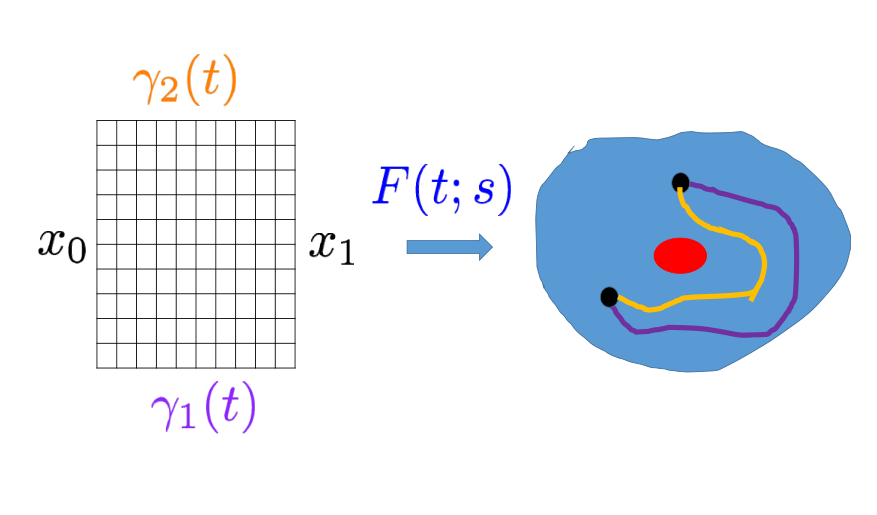
\includegraphics[width=0.72\textwidth]{figures/fig35.png}
  \caption{用图示说明下述论证：在 $\mathbb{C}$ 的一个区域上，平坦联络的平行移动只依赖固定端点曲线所在的同伦类。
  利用该同伦，把两条曲线之间的区域划分成小块：只需把同伦的定义域剖分成足够小的方块。
  于是绕每个小方块的单值性由联络及其协变导数算出，而这些全都为零。（原文 Fig.~35，第 207 页）}
  \label{fig:35}
\end{figure}

\textbf{例 3}\quad 设 $B$ 是 $\mathbb{C}$ 中的开连通区域。例如 $B$ 可以是
$\mathbb{C}-\{z_1,\dots,z_m\}$，即 $\mathbb{C}$ 去掉某组点。我们也可以把它看成扩充复平面再去掉
无穷远点：$B=\mathbb{C}P^1-\{z_1,\dots,z_m,\infty\}$。因此当 $m\ge 1$ 时它绝对不单连通。
再令 $E=B\times\mathbb{C}^n$，其中 $n$ 为某正整数。$B$ 中的路径可以用 $z(t)$ 表示。我们的路径提升规则
与例 1 类似：在 $B$ 上选取一对 $n\times n$ 矩阵值函数，记作 $(A_z,A_{\bar z})$，其中这一对里的每个矩阵
都是 $(z,\bar z)$ 的单值非奇异函数。\footnote{我们并不假定复共轭 $(A_z)^*$ 与 $A_{\bar z}$ 之间有任何关系。}
于是提升路径将是 $(z(t),\vec{v}(t))$，其中微分方程现在为：

\begin{equation}
  \frac{d}{dt}\vec{v}(t) + \left(A_z(z(t),\bar z(t))\frac{dz}{dt}
  + A_{\bar z}(z(t),\bar z(t))\frac{d\bar z}{dt}\right)\vec{v}(t) = 0
  \qquad \vec{v}(0)=\vec{v}_0.
  \tag{H.23}
  \label{eq:H.23}
\end{equation}

我们同样可以用路径排序指数「解出」这个微分方程，同样会有相当有趣的单值性。注意我们把两项放在了
方程的同一侧（因而这里的 $A$ 与前几个例子相差一个符号翻转）。这一符号约定最终更有用。

作为单值性的例子，让我们考虑以 $z_0$ 为基点的小环路，写成 $z(t)=z_0+\epsilon(t)$，其中对固定的 $t$，
复数 $\epsilon(t)$ 取得很小。特别地，该环路是同伦平凡的，于是存在以 $z_0$ 为基点的、使 $\partial D$
为 $\wp$ 的像的小圆盘 $D$。此时 $\mathbb{U}(\wp)$ 的首个非平凡贡献出现在 $\mathcal{O}(\epsilon^2)$ 阶，
并且可以证明

\begin{equation}
  \mathbb{U}(\wp) = 1 + \alpha F_{z\bar z}(z_0,\bar z_0) + \mathcal{O}(\epsilon^3)
  \tag{H.24}
  \label{eq:H.24}
\end{equation}

其中

\begin{equation}
  \alpha = \int_0^1 dt\,\dot{\epsilon}(t)\bar{\epsilon}(t)
  \tag{H.25}
  \label{eq:H.25}
\end{equation}

是（$(2i)$ 倍的）以 $z_0$ 处小环路所围的欧氏面积，而

\begin{equation}
  F_{z\bar z} := \partial_z A_{\bar z} - \partial_{\bar z}A_z + [A_z,A_{\bar z}]
  \tag{H.26}
  \label{eq:H.26}
\end{equation}

看清 $\alpha$ 正比于环路所围面积的一个办法是把它写成

\begin{equation}
  \alpha = \oint_\wp d\epsilon\,\bar{\epsilon} = \int_D d\epsilon\wedge d\bar{\epsilon}
  \tag{H.27}
  \label{eq:H.27}
\end{equation}

而后一个积分是环路所围欧氏面积的 $2i$ 倍。可以证明：在 \eqref{eq:H.24} 按 $\epsilon(t)$ 的幂作完整展开时，
所有项都只涉及 $\mathbb{F}_{z\bar z}$ 及其（协变）导数的乘积。

% [Tutor Note: (H.24) 与 (H.31) 的符号相反不要当成矛盾，(H.24) 的 $+$ 与 (H.31) 的 $-$ 来自
%  (H.23) 把两项移到方程同侧、即 $A$ 相对例 1 差一个符号，而 (H.29) 又沿用了 (H.23) 的约定；
%  核对时请从 (H.23) 的 $+\dot{v}+A\dot{x}v=0$ 出发重算一遍 $\epsilon$ 的一阶展开，否则很容易
%  把 $F$ 的整体符号搞反。另外 (H.25) 的 $\alpha$ 只取了「面积」的一阶项，
%  $\oint d\epsilon\,\bar\epsilon$ 与 $\int_D d\epsilon\wedge d\bar\epsilon$ 相差一个由 Stokes 定理
%  保证的边界项，故 $\alpha=2i\cdot\text{面积}$ 成立的前提是 $D$ 上 $\epsilon$ 单值。
%  另外 (H.32) 中 $[A_\mu,A_\nu]$ 的次序也必须与 $\partial_\mu A_\nu-\partial_\nu A_\mu$
%  的反对称性一致：把两项同时反号（$\mu\leftrightarrow\nu$）才自洽，别只改其中一项。]

% 说明：原文这一句写的是 "all the terms involve products of $\mathbb{F}_{z\bar z}$"，
%  用的是黑板粗体 $\mathbb{F}$ 而不是 $F$；这是作者笔误（同一页 (H.26) 用的是 $F_{z\bar z}$），
%  此处照原样转写，阅读时按 $F_{z\bar z}$ 理解。

{\small\itshape ［原文标记：这一点需要更充分地论证。］}

% [原文待办标记，原文 p.208 右侧页边 \ensuremath{\clubsuit}Need to justify that more fully. \ensuremath{\clubsuit}]

表达式 $F_{z\bar z}$ 称为该联络的曲率（curvature）。更恰当地，应把它看成本地矩阵值的 2-形式
$F=F_{z\bar z}dz\wedge d\bar z$。

有一类特别重要的联络是\emph{平坦联络}（flat connection），定义为曲率为零的联络。此时，给定平坦联络，
闭路的单值性矩阵 $\mathbb{U}(\wp)$ 只依赖 $\wp$ 在 $B$ 中的同伦类。用 \eqref{eq:H.24} 与路径复合性质很容易
证明这一点。由 \eqref{eq:H.24}，绕小环路的单值性必须是平凡的。而若 $F(t;s)$ 是从闭路 $\wp_1(s)$ 到
$\wp_2(s)$ 的同伦，则我们可以把方块 $I^2$ 剖分成许多小方块，绕每个小方块的单值性都必须是平凡的，
因此绕整个方块的单值性也必须是平凡的。于是 $\mathbb{U}(\wp_1\star\bar{\wp}_2)=1$，从而
$\mathbb{U}(\wp_1)=\mathbb{U}(\wp_2)$。

{\small\itshape ［原文标记：需要更多解释］}

% [原文待办标记，原文 p.208 右侧页边 \ensuremath{\clubsuit}Need more explanation \ensuremath{\clubsuit}；正文该句「绕每个小方块的
%  单值性都必须是平凡的」的前提是小方块内部没有奇点，这正是「平坦」的用处，作者未明说。]

在 $A_{\bar z}=0$ 且 $A_z$ 是 $z$ 的全纯函数这一特殊情形下，「$\mathbb{U}(\wp)$ 只依赖同伦类」
这一性质可以直接从路径排序指数看出来：

\begin{equation}
  \begin{aligned}
    \mathbb{U}(\wp_t) = {}& 1 + \int_{z_0}^{z(t)} A(z_1)dz_1 \\
    &+ \sum_{n=2}^{\infty}\int_{z_0}^{z(t)} dz_1\int_{z_0}^{z_1}dz_2\cdots\int_{z_0}^{z_{n-1}}dz_n\,
      A(z_1)\cdots A(z_n)
  \end{aligned}
  \tag{H.28}
  \label{eq:H.28}
\end{equation}

而此时该断言由 Cauchy 定理推出。这里 $dz_i$ 是 $\dot{z}(t_i)dt_i$ 等的简写。

\begin{figure}[htbp]
  \centering
  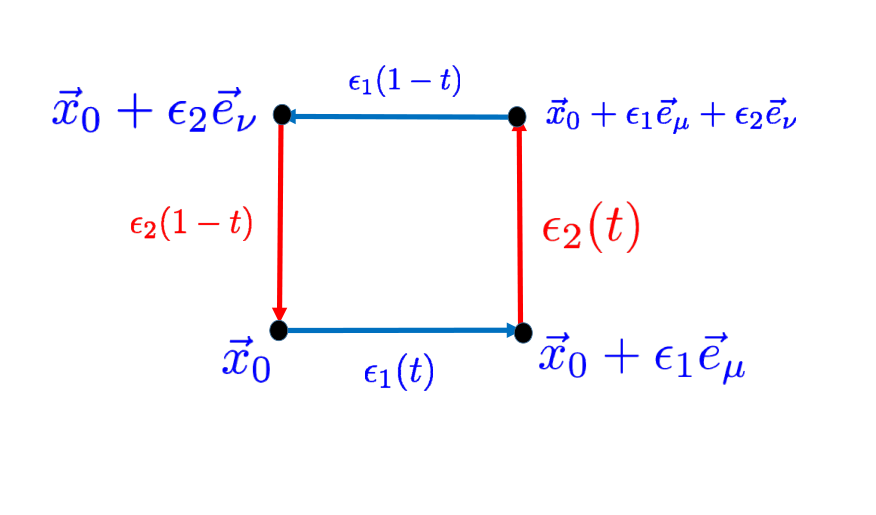
\includegraphics[width=0.60\textwidth]{figures/fig36.png}
  \caption{当 $\epsilon_1$ 与 $\epsilon_2$ 很小时，单值性的全部贡献都来自联络的曲率，
  其首项由环路的面积乘以 $\vec{x}_0$ 处由该环路（在切空间中）张成的平面内的曲率分量决定。
  （原文 Fig.~36，第 209 页）}
  \label{fig:36}
\end{figure}

\textbf{例 4}\quad 现在取 $B$ 为 $\mathbb{R}^m$ 中的开区域（$m>0$ 任意），$E=B\times\mathbb{C}^N$，
其中 $m$ 与 $N$ 一般完全无关。在 $\mathbb{C}^N$ 上取坐标 $x^\mu$，$\mu=1,\dots,m$，并令 $A_\mu(x)$
是 $B$ 上 $m$ 个复 $N\times N$ 矩阵值函数。我们假定它们单值且非奇异。与上面几个例子非常类似，
这些数据足以在由到第一个因子的投影给出的纤维化 $p:E\to B$ 上定义一个联络：设
$\wp:[0,1]\to B$ 是 $B$ 中从 $\vec{x}_0$ 到 $\vec{x}_1$ 的（分段可微）路径。然后我们在 $\vec{x}_0$
上方的纤维中选取提升 $(\vec{x}_0,\vec{v}_0)\in E$，并求解微分方程

\begin{equation}
  \frac{d}{dt}\vec{v}(t) + A_\mu(\vec{x}(t))\frac{dx^\mu(t)}{dt}\vec{v}(t) = 0
  \qquad \vec{v}(0)=\vec{v}_0
  \tag{H.29}
  \label{eq:H.29}
\end{equation}

而 $\mathbb{P}(\wp)(t)=(\vec{x}(t),\vec{v}(t))$ 就是提升。一般地会有有趣的单值性，甚至在任意点
$\vec{x}_0$ 附近的同伦平凡小路径上就已经出现。相关表达式是 \eqref{eq:H.24} 与 \eqref{eq:H.26} 的简单推广。确实，
任何无穷小曲线都可以看成落在某个过 $\vec{x}_0$ 的平面内，于是只需从复坐标换回实坐标即可。
或者，我们可以考虑由绕过 $x^\mu$-$x^\nu$ 平面内一个方形的四条开路径复合而成的小路径：

\begin{equation}
  \begin{aligned}
    \wp_1(t) &= \vec{x}_0 + \epsilon_1(t)\vec{e}_\mu \\
    \wp_2(t) &= (\vec{x}_0 + \epsilon_1\vec{e}_\mu) + \epsilon_2(t)\vec{e}_\nu \\
    \wp_3(t) &= (\vec{x}_0 + \epsilon_2\vec{e}_\nu) + \epsilon_1(1-t)\vec{e}_\mu \\
    \wp_4(t) &= \vec{x}_0 + +\epsilon_2(1-t)\vec{e}_\nu
  \end{aligned}
  \tag{H.30}
  \label{eq:H.30}
\end{equation}

% [Tutor Note: (H.30) 第四行原文多打了一个加号（$\vec{x}_0++\epsilon_2(1-t)\vec{e}_\nu$），
%  是排版笔误，此处照原样保留，数学上应读作 $\vec{x}_0+\epsilon_2(1-t)\vec{e}_\nu$。
%  另外 $\wp_4$ 的终点必须回到 $\vec{x}_0$ 才能闭合，故该行里的 $+ +$ 若按字面理解会破坏闭合性，
%  这也印证它是笔误。]

于是 $\wp=\wp_1\star\wp_2\star\wp_3\star\wp_4$。这里 $\vec{e}_\mu$ 是指向 $x^\mu$ 方向的单位向量，
而 $\epsilon_i:=\epsilon_i(t=1)$。见图 36。一个简单的计算表明 \eqref{eq:H.24} 与 \eqref{eq:H.26} 被推广为

\begin{equation}
  \mathbb{U}(\wp) = 1 - \epsilon_1\epsilon_2 F_{\mu\nu}(\vec{x}_0) + \cdots
  \tag{H.31}
  \label{eq:H.31}
\end{equation}

\begin{equation}
  F_{\mu\nu} := \partial_\mu A_\nu - \partial_\nu A_\mu + [A_\mu,A_\nu]
  \tag{H.32}
  \label{eq:H.32}
\end{equation}

而 \eqref{eq:H.31} 中的高阶项都是 $\epsilon_1^a\epsilon_2^b$ 阶的，其中 $a>0$、$b>0$、$a+b>2$。

\textbf{注}：可以证明，\eqref{eq:H.31} 中高阶项的系数是 $F_{\mu\nu}$ 及其沿 $\mu$ 与 $\nu$ 方向的协变导数的
多项式。一般地，任一矩阵值函数 $\Phi(x)$ 沿 $\lambda$ 方向的协变导数为

\begin{equation}
  D_\lambda\Phi := \partial_\lambda\Phi + [A_\lambda,\Phi]
  \tag{H.33}
  \label{eq:H.33}
\end{equation}

{\small\itshape ［原文标记：这一点有简单证明吗？或者有生成该级数的办法吗？我猜它是
$e^{\epsilon_1 D_\mu}e^{\epsilon_2 D_\nu}e^{-\epsilon_1 D_\mu}e^{-\cdots}$］}

% [原文待办标记，原文 p.210 右侧页边 \ensuremath{\clubsuit}Is there a simple proof of that? Or a way to generate
%  the series? I am guessing it is e^{ε1D_μ}e^{ε2D_ν}e^{-ε1D_μ}e^{-…} \ensuremath{\clubsuit} —— 作者的猜测正是
%  把 (H.30) 的方形环路写成四个平行移动算符的乘积，再作 BCH 展开。]

% 说明：(H.31) 里的负号与 (H.24) 里的正号之所以不同，见 (H.23) 之后的说明；若按例 1 的
%  约定 $\dot{v}=A\dot{x}v$（无负号）重算 (H.30) 的方形环路，得到的是
%  $\mathbb{U}=1+\epsilon_1\epsilon_2F_{\mu\nu}$。

\paragraph{练习}
对 $B=\mathbb{C}^*$、$N=1$、$A_z=\frac{\mu}{z}$、$A_{\bar z}=0$ 求解 \eqref{eq:H.23}，其中 $\mu$ 是复数。
计算该联络绕 $B$ 中某些简单闭路的单值性。

\paragraph{练习}
给出方程 \eqref{eq:H.24}、\eqref{eq:H.26}、\eqref{eq:H.31} 与 \eqref{eq:H.32} 的仔细推导。

\paragraph{练习}
证明：若矩阵 $A_\mu(x)$ 是反 Hermite 的，即 $(A_\mu(x))^{\dagger}=-A_\mu(x)$，则

\begin{equation}
  \mathrm{Pexp}\int_0^t A_\mu(x(t_1))\frac{dx^\mu}{dt_1}dt_1
  \tag{H.34}
  \label{eq:H.34}
\end{equation}

是酉的。

\paragraph{练习：规范变换}
设 $A(x)$ 是 $\mathbb{R}$ 上取值 $n\times n$ 复矩阵的矩阵值函数，而 $x\mapsto g(x)$ 是从 $\mathbb{R}$
到 $GL(n,\mathbb{C})$ 的可微映射。用

\begin{equation}
  A(x) = g(x)^{-1}\widetilde{A}(x)g(x) + g(x)^{-1}\frac{d}{dx}g(x)
  \tag{H.35}
  \label{eq:H.35}
\end{equation}

定义一个矩阵值函数 $\widetilde{A}(x)$。

% 说明：该练习的 a.)--f.) 各小问在下一页（印刷第 211 页），属下一片段；本片段止于 (H.35)。
